%\title{Overleaf Memo Template}
% Using the texMemo package by Rob Oakes
\documentclass[a4paper,11pt]{article}
\usepackage[english]{babel}
\usepackage{graphicx, lipsum}
\usepackage{graphics} % for pdf, bitmapped graphics files
\usepackage{epsfig} % for postscript graphics files
\usepackage{amsmath} % assumes amsmath package installed
\usepackage{amssymb}  % assumes amsmath package installed
% \usepackage{multirow}
\usepackage{url}

%% Edit the header section here. To include your
%% own logo, upload a file via the files menu.
\title{Problem Set 1 \\ \Large Advanced Methods in Applied Statistics}

\author{Magnus Berg Sletfjerding}
\date{\today}

\begin{document}
\maketitle

\section{Exercise 1}
For the first part of the assignment, I used scrapy ( \url{https://scrapy.org/}) to parse the data on the given website to a csv.

The main challenge lay in figuring out the fact that teams without a seed had two (!) fewer columns.
This took longer than I care to admit, but I extracted all the data into csv files. (attached)

I treated the data with pandas dataframes, and plotted the data in figure \ref{exc1}.

\begin{figure}[ht!]
  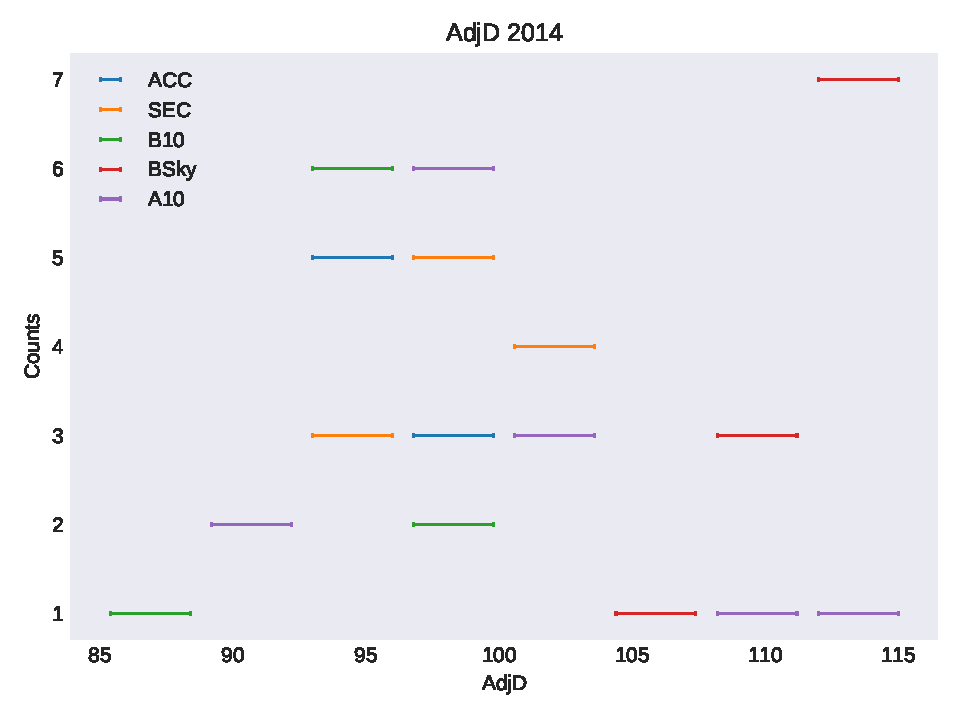
\includegraphics[width=\linewidth]{../plots/Exc1.pdf}
  \caption{Exercise 1 - histogram of all the teams}
  \label{exc1}
\end{figure}


\section{Exercise 2}
Importing this csv took three clicks.
Thanks for the tip on code robustness, Jason.

With Pandas, subtracting the two columns was simple enough.
Eliminating NaN values was also straightforward.

This resulted in figure \ref{exc2}.

\begin{figure}[ht!]
  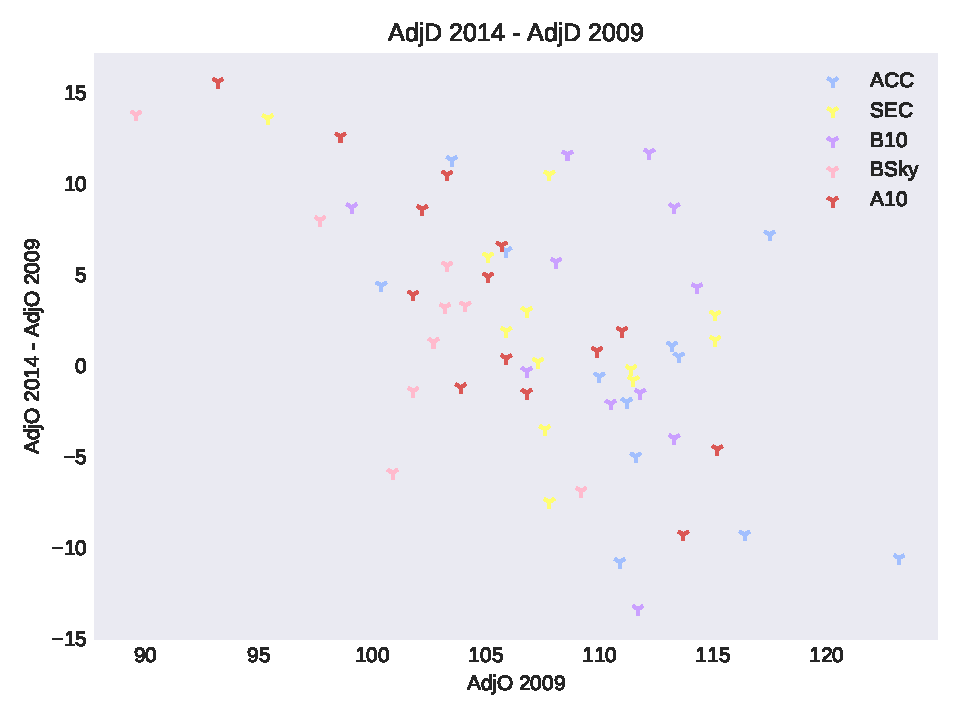
\includegraphics[width=\linewidth]{../plots/Exc2.pdf}
  \caption{Exercise 2 - plot of the AdjO of all the teams as fcn of 2009 AdjO}
  \label{exc2}
\end{figure}

Pandas' mean and median functions also came in handy here, and I generated the following .txt file.

AdjO-diff-Md is Median, while AdjO-diff-Mn is Mean

\begin{verbatim}
  Conference   AdjO diff-Md
  ACC                 -0.05
  SEC                  1.65
  B10                  4.30
  BSky                 3.20
  A10                  2.90
  Outsiders            1.30
  Conference   AdjO diff-Mn
  ACC                 -0.63
  SEC                  2.28
  B10                  2.67
  BSky                 2.32
  A10                  3.51
  Outsiders            2.40
\end{verbatim}






\section{Exercise 3}

Again, Jason's tip about robust and scalable code came in handy.

\subsection{Exercise 1 redone}


\begin{figure}[ht!]
  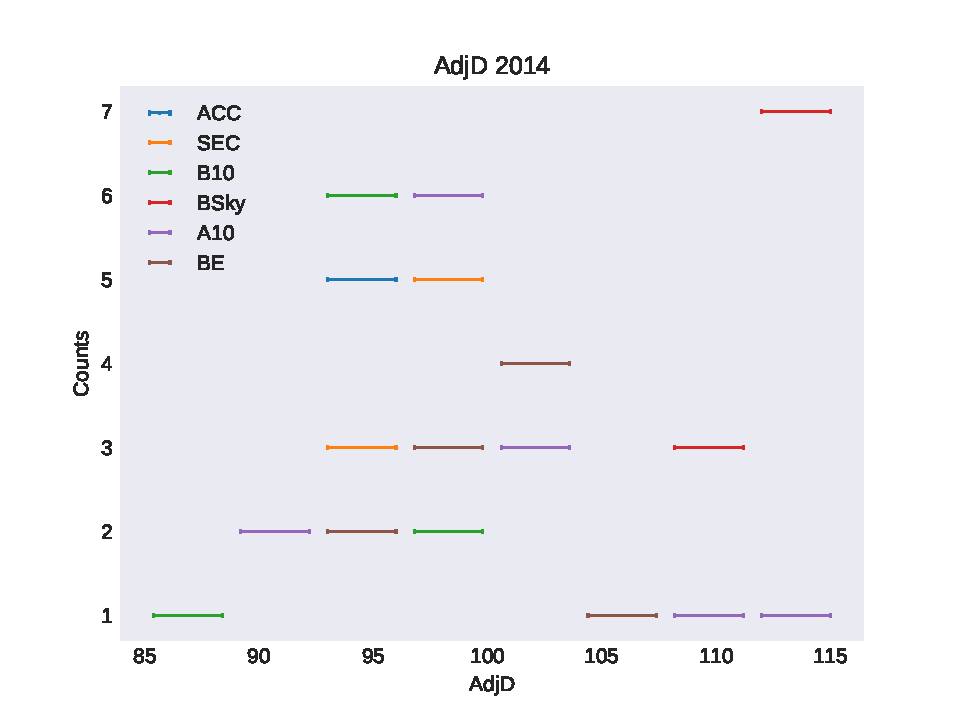
\includegraphics[width=\linewidth]{../plots/Exc31.pdf}
  \caption{Exercise 3-1 - histogram of all the teams}
  \label{exc31}
\end{figure}

\subsection{Exercise 2 redone}


\begin{figure}[ht!]
  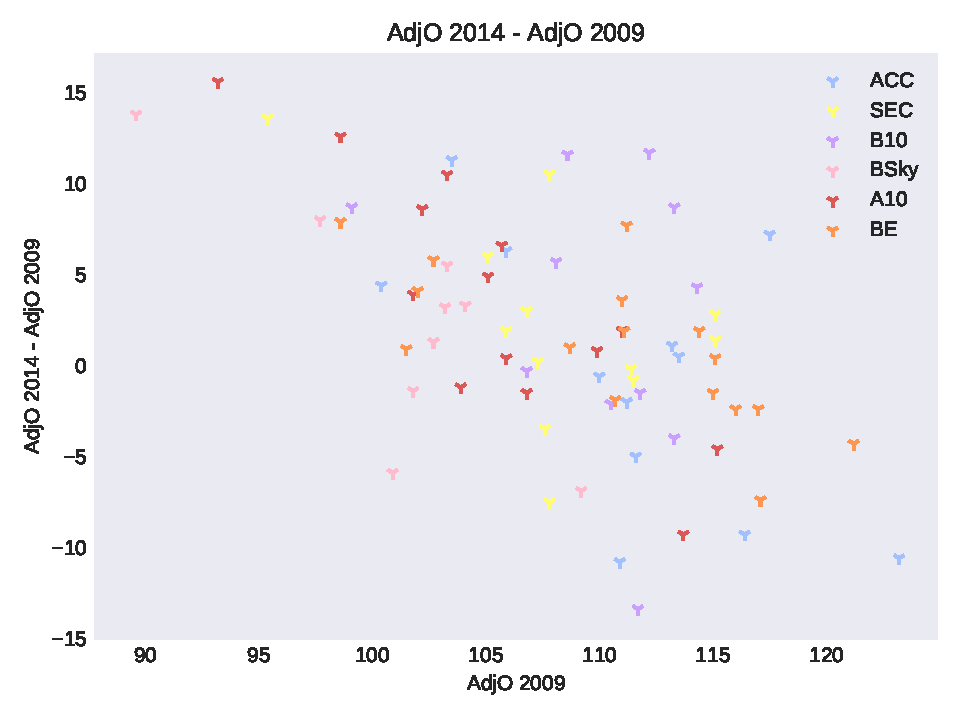
\includegraphics[width=\linewidth]{../plots/Exc32.pdf}
  \caption{Exercise 3-2 - plot of the AdjO of all the teams as fcn of 2009 AdjO}
  \label{exc2}
\end{figure}

Another text file was generated:

\begin{verbatim}
  Conference   AdjO diff-Md
  ACC                 -0.05
  SEC                  1.65
  B10                  4.30
  BSky                 3.20
  A10                  2.90
  BE                   0.95
  Outsiders            1.50
  Conference   AdjO diff-Mn
  ACC                 -0.63
  SEC                  2.28
  B10                  2.67
  BSky                 2.32
  A10                  3.51
  BE                   0.96
  Outsiders            2.49
\end{verbatim}

\end{document}
